\documentclass{article}
\usepackage[utf8]{inputenc}
\usepackage{bm}
\usepackage{../../lib/approx-scribe}

\usepackage[T1]{fontenc}

\allowdisplaybreaks

\begin{document}

\lecture{11}{Ball-Growing and Multicut}{Antares Chen}{5/10/2019}


% --------------------------------------------------------------------
% INTRODUCTION
% --------------------------------------------------------------------
Last time, we alluded that the spectrum of the Laplacian allows us to continuously measure combinatorial properties of a graph. We will make this statement precise by introducing a notion of connectivity called graph conductance. This will lead us to Cheeger's isoperimetric inequality which relates graph conductance to the second smallest eigenvalue of the normalized Laplacian.



% --------------------------------------------------------------------
% MULTICUT PROBLEM + RELAXATION
% --------------------------------------------------------------------
\section{Multicut and its Linear Programming Relaxations}

Given a graph $G = (V, E)$, edge costs $c_e \geq 0$, and a set of source-sink vertex pairs $\{ (s_i, t_i): i = 1, \ldots, k \}$, the multicut problem asks for $F \subseteq E$ that, when removed, separates each $s_i, t_i$ with minimal cost according to
\begin{equation*}
\textup{cost}(F) = \sum_{e \in F} c_e
\end{equation*}

The multicut problem is not only $\NP$-hard in general, but is also $\NP$-hard when $G$ is restricted to be a trees. It is also known to be $\APX$-hard due to a reduction to the Unique Games Conjecture~\cite{CKKRS06}.

\begin{theorem}
Assuming the Unique Games Conjecture, there does not exist an $\alpha$-approximation for multicut for any $\alpha \geq 1$ unless $\ClassP = \NP$.
\end{theorem}

A stronger version of the Unique Games Conjecture demonstrates that there does not exist an $O(\log \log n)$ approximation unless $\ClassP = \NP$. It is currently an open problem to design an approximation algorithm that matches the lower bound. For these notes, we will present a $4\ln(k+1)$-approximation algorithm due to Garg, Vazirani, and Yannakakis. The algorithm first performs a linear programming relaxation, then rounds the solution using a procedure known as \emph{ball-growing} which is applicable as the LP relaxation benefits from certain \emph{metric} properties. Let us first construct a easily interpretable LP relaxation whose metric properties are not immediately evident.

% --------------------------------------------------------------------
% A PATH-BASED LP RELAXATION
% --------------------------------------------------------------------

\subsection{A Path-Based LP Relaxation}

We begin with the multicut integer program. First, define decision variables for each edge $e$.
\begin{equation*}
x_e = \begin{cases}
1 & \text{if }e \text{ is removed} \\
0 & \text{otherwise}
\end{cases}
\end{equation*}

Our objective is then to minimize the cost of $F$. The objective function is
\begin{equation*}
\text{cost}(F) = \sum_{e \in E} c_e x_e
\end{equation*}

Finally, we must constrain our integer program to return an assignment that cuts each $s_i$ and $t_i$ pair. We know that $s_i$, $t_i$ are cut by $F$ if an edge on each path between the two vertices is removed. Let $\mathcal{P}_i$ be the set of all $s_i$ to $t_i$ paths. It suffices for us to ensure that at least one edge admits $x_e = 1$ for every $P \in \mathcal{P}_i$. This is equivalent to adding the constraints
\begin{equation*}
\sum_{e \in P} x_e \geq 1
\qquad \forall P \in \mathcal{P}_i \quad \forall i = 1, \ldots, k
\end{equation*}

This gives our integer program. The linear programming relaxation of this replaces the integrality constraint with $x_e \geq 0$. The LP relaxation for multicut is then the following.
\begin{equation}\label{eq:primal-lp}
\begin{aligned}
& \text{minimize}
& & \sum_{e \in E} c_e x_e & \\
& \text{subject to}
& & \sum_{e \in P} x_e \geq 1 & & \forall P \in \mathcal{P}_i & & \forall i = 1, \ldots, k \\
& & & x_e \geq 0 & & \forall e \in E
\end{aligned}
\end{equation}

An algorithm that rounds this LP will first need to solve for $x_e$. But there is an immediate issue: there could be exponentially many path constraint with respect to the size of the graph! There are two ways to get around this. First is to derive an alternative LP relaxation that has polynomially many constraints, while second is to employ the \emph{Ellipsoid Method}, a procedure that can solve exponentially sized linear programs provided that one can demonstrate the existence of a \emph{separation oracle}. We'll instead demonstrate a polynomially sized, relaxation for multicut that more clearly highlights the metric structure that exists in multicut.

% --------------------------------------------------------------------
% A METRIC LP RELAXATION
% --------------------------------------------------------------------

\subsection{A Metric LP Relaxation}

Consider a valid multicut $F$ and define the indicator function $d_{F}: V \times V \rightarrow \{ 0, 1 \}$ on pairs of vertices that are separated when $F$ is removed.
\begin{equation*}
d_F(u, v) = \begin{cases}
1 & \text{ if } u \text{ and } v \text{ are separated by } F \\
0 & \text{otherwise}
\end{cases}
\end{equation*}

This function defines a \emph{metric}\footnote{Actually, $d_F$ is called a semi-metric as $d_F(u, v) = 0$ does not necessarily imply $u = v$ as usually required by metrics.} over pairs of vertices in $G$. It holds that $d_F(u, u) = 0$ for any vertex $u$, is non-negative, symmetric, and satisfies the triangle inequality. To see that $d_F$ satisfies the triangle inequality, consider any three distinct vertices $u, v, w$. Since distances are $\{ 0, 1 \}$, we need only verify that the triangle with two sides 0 never exists. It cannot exist because any cut which separates two of $u, v, w$ must remove two sides of the triangle.

The function $d_F$ is often called the \emph{cut metric} induced by the partition. It is a 0-1 metric defined over all pairs of vertices. The multicut problem thus asks for the minimum cost metric among all cut metrics separating each $s_i$, $t_i$ pair. A valid relaxation of this problem would then be to ask for the minimum cost metric among \emph{all metrics} separating each $s_i$, $t_i$ pair. To formulate this relaxation as a linear program, we begin by noting that the metric constraints can be encoded via linear expressions. If $x_{uv}$ denotes the distance between two vertices $u, v$, we can write the constraints as
\begin{equation*}
\begin{aligned}
& x_{uv} + x_{vw} \geq x_{uw} & & \forall u \neq v \neq w & & \text{triangle inequality} \\
& x_{uv} = x_{vu} & & \forall u, v \in V & & \text{symmetry} \\
& x_{uv} \geq 0 & & \forall u, v \in V & & \text{non-negativity}
\end{aligned}
\end{equation*}

Next, to enforce that the metric separates each $s_i$, $t_i$ pair, we need only to ensure that the distance between the source and sink is at least 1. For each $i$, we add the constraint $x_{s_i, t_i} \geq 1$. We can thus write the following \emph{metric} LP relaxation for multicut.
\begin{equation}\label{eq:metric-lp}
\begin{aligned}
& \text{minimize}
& & \sum_{u, v \in V} c_{uv} x_{uv} & \\
& \text{subject to}
& & x_{uv} + x_{vw} \geq x_{uw} & & \forall u \neq v \neq w \\
& & & x_{s_i, t_i} \geq 1 & & \forall i = 1, \ldots, k \\
& & & x_{uv} \geq 0 & & \forall u, v \in V
\end{aligned}
\end{equation}

Note we need not write the symmetry constraint as the edge costs are symmetric. It is worth checking that this is a valid relaxation of multicut.

\begin{claim}\label{claim:metric-valid}
Let $x$ be an integral solution to LP~\ref{eq:metric-lp}. Then removing any $e$ where $x_{e} = 1$ removes a valid multicut.
\end{claim}
\begin{proof}
Suppose not; then there is a pair $s_i, t_i$ with a path $P$ such that each edge $e \in P$ admits $x_e = 0$. Intuitively, this violates the triangle inequality as the direct distance $x_{s_i, t_i}$ should be the shortest distance between $s_i, t_i$ of which the constraint $x_{s_i, t_i} \geq 1$ dictates must be at least 1.

More precisely, imagine a new graph $G'$ constructed from $G$ with its edges weighted by $x_e$. We claim that $x_{s_i, t_i}$ denotes the shortest path distance between $s_i, t_i$ in $G'$. Consider any other $s_i, t_i$ path $P$ and write it as
\begin{equation*}
s_i
\quad u_1
\quad \ldots
\quad u_\ell
\quad t_i
\end{equation*}

Now, the triangle inequality allows us to write a sequence of inequalities like so
\begin{equation*}
x_{s_i, u_1} + x_{u_1, t_i} \geq x_{s_i, t_i}
\qquad\qquad
x_{u_1, u_2} + x_{u_2, t_i} \geq x_{u_1, t_i}
\qquad\qquad
\ldots
\qquad\qquad
x_{u_{\ell - 1}, u_\ell} + x_{u_\ell, t_i} \geq x_{u_{\ell - 1}, t_i}
\end{equation*}

Together, these inequalities imply the following relation
\begin{equation*}
x_{s_i, u_1} + x_{u_1, u_2} + \ldots + x_{u_{\ell - 1}, u_\ell} + x_{u_\ell, t_i} \geq x_{s_i, t_i}
\end{equation*}

The LHS is the length of $P$ while the RHS is the weight of the edge $(s_i, t_i)$ in $G'$. Thus the length of any $s_i, t_i$ path in $G'$ must be at least $x_{s_i, t_i}$. Now, if there is a path $P$ such that $x_e = 0$ for $e \in P$ then its length in $G'$ is 0 contradicting the fact that the shortest $s_i, t_i$ path must have length at least 1.
\end{proof}

One thing to note about this relaxation is that the metric is defined over all pairs of vertices, but the given graph may not have an edge between each vertex pair. It suffices to let $c_{uv} = 0$ whenever $(u, v) \notin E$ as cutting an edge that does not exist in the graph does not contribute to the cost of the cut.

\subsection{Metric Completions}

Given a solution to LP~\ref{eq:metric-lp}, we can construct an alterate LP solution by performing a \emph{metric completion}. For every pair of vertices $u, v \in V$, the metric completion of $x$ assigns $\hat{x}_{uv}$ to be the length of the shortest path between $u$ and $v$ in the graph $G$ whose edges $e$ are weighted as $x_e$. That is if we denote $\mathcal{P}_{uv}$ as the set of all paths from $u$ to $v$, $\hat{x}_{uv}$ is given by
\begin{equation*}
\hat{x}_{uv} = \min_{P \in \mathcal{P}_{uv}} \sum_{e \in P} x_e
\end{equation*}

Notice that $\hat{x}_{uv}$ is both a feasible and optimal solution for LP~\ref{eq:metric-lp}.

\begin{claim}\label{claim:metric-completion}
Given a solution $x$ to LP~\ref{eq:metric-lp}, its metric completion $\hat{x}$ is feasible and optimal.
\end{claim}
\begin{proof}
Notice that $\hat{x}_{uv}$ automatically forms a metric between all pairs of vertices as shortest path distances satisfy the triangle inequality. Thus to demonstrate feasibility, we need only verify that $\hat{x}_{s_i, t_i} \geq 1$ for each $i$. However, the argument for claim~\ref{claim:metric-valid} demonstrates that $\hat{x}_{s_i, t_i} = x_{s_i, t_i} \geq 1$ since $x_{s_i, t_i}$ is the shortest path length between $s_i, t_i$ in a graph weighted by $x_e$'s.

To demonstrate optimality, notice that the objective value of $\hat{x}$ is equivalent to that of $x$. For any $e \in E$, we have that $\hat{x}_e \leq x_e$. This is because $\hat{x}_e$ is the length of the shortest path between the endpoints of $e$. Taking just the edge $e$ is one such path, thus the length of the shortest path can only be shorter than $x_e$. Consequently, the objective value of $\hat{x}$ is at most
\begin{equation*}
\sum_{e \in E} c_e \hat{x}_e \leq \sum_{e \in E} c_e x_e
\end{equation*}

Because $x$ is an optimal solution to the LP, $\hat{x}$ must be an optimal solution as well.
\end{proof}

Optimality in claim~\ref{claim:metric-completion} actually follows for a simpler reason -- $\hat{x}_e = x_e$ for any $e \in E$ thus the two objective values are in fact equal. The reason why the above argument is provided is because it also applies to demonstrating that the metric completion of a solution to the path-based relaxation~\ref{eq:primal-lp} is optimal and feasible for LP~\ref{eq:primal-lp}.

In fact, performing a metric completion tells us how to relate the above two LP relaxations together since the completion of a solution to either LP makes it feasible for the other. The metric completion of a solution to the metric relaxation~\ref{eq:metric-lp} is feasible for the path-based LP~\ref{eq:primal-lp} because it will satisfy the following constraints:
\begin{equation*}
\sum_{e \in P} \hat{x}_e \geq 1
\qquad\qquad\qquad\qquad
\forall P \in \mathcal{P}_i \; \forall i = 1, \ldots, k
\end{equation*}

The metric relaxation requires $x_{s_i, t_i} \geq 1$. The value of $x_{s_i, t_i}$ is also the shortest path length between $s_i, t_i$. Thus any other path must have length at least 1. In the other direction, we can show that the metric completion of $x$ the solution to the path-based LP relaxation~\ref{eq:primal-lp} is also a feasible and optimal solution for that LP. It is then feasible for LP~\ref{eq:metric-lp} as shortest path distances automatically satisfy the triangle inequality, and $\hat{x}_{s_i, t_i} \geq 1$ for all $i$ because $\sum_{e \in P} x_e \geq 1$ for any path $P$ between $s_i, t_i$.



% --------------------------------------------------------------------
% ROUNDING ALGORITHM + CORRECTNESS
% --------------------------------------------------------------------
\section{Rounding the Linear Program}

We will now develop an algorithm for rounding a solution $x$ to the metric LP relaxation~\ref{eq:metric-lp}. Let's start by addressing how to construct a \emph{valid} multicut, then determine how to make it \emph{low-cost}. For the remainder of these notes, we'll denote $d_x(u, v)$ as the metric completion of $x$ on edge $(u, v)$.

% --------------------------------------------------------------------
% BALLS AND PIPE SYSTEMS
% --------------------------------------------------------------------

\subsection{Balls and Pipe Systems}

We want to leverage the metric structure from our LP relaxation to construct our multicut. One way to do this is to partition the graph into clusters separating each $s_i, t_i$ pair, then remove the multicut consisting of edges that cross the boundary of each cluster. We can use the fact that $d_x$ is a metric to construct our clusters by choosing balls of a certain radius as measured by $d_x$. Let's define the ball of radius $r$ centered at vertex $u' \in V$ as $\mathcal{B}_x(u', r) \subseteq V$, the set of all vertices within distance $r$ of $u'$ as measured by the distance $d_x$.
\begin{equation*}
\mathcal{B}_x(u', r) = \{ v \in V : d_x(u', v) \leq r \}
\end{equation*}

Later on, it will be useful for us to consider the \emph{volume} of each ball. Given $S \subseteq V$, let $E(S)$ denote the set of edges whose endpoints are contained in $S$. Additionally, let $\partial(S)$ denote the set of edges on the \emph{boundary} of $S$, i.e. $(u, v)$ with $u \in S$ and $v \notin S$. The volume of a ball $\mathcal{B}_x(u', r)$ is defined by the following:
\begin{equation*}
\text{Vol} \; \mathcal{B}_x(u', r)
= \sum_{e \in E(\mathcal{B}_x(u', r))} c_e x_e + \sum_{(u, v) \in \partial(\mathcal{B}_x(u', r)) : u \in \mathcal{B}_x(u', r)} c_{uv} \big( r - d_x(u', u) \big)
\end{equation*}

Williamson and Shmoy's \emph{The Design of Approximation Algorithms} uses the analogy of a \emph{pipe system} to interpret these definitions. We think of the graph as a network of pipes: each edge $e$ is replaced with a pipe of \emph{length} $x_e$ and \emph{cross sectional area} $c_e$. The term $c_e x_e$ then denotes the volume of the pipe replacing $e$. The quantity $\text{Vol} \; \mathcal{B}_x(u, r)$ could then be interpreted as the total volume of all pipes within a radius $r$ of $u$.
\begin{equation*}
\text{Vol} \; \mathcal{B}_x(u', r)
= \underbrace{\sum_{e \in E(\mathcal{B}_x(u', r))} c_e x_e}_\text{Total volume of pipe contained in the ball}
+ \underbrace{\sum_{(u, v) \in \partial(\mathcal{B}_x(u', r)) : u \in \mathcal{B}_x(u', r)} c_{uv} \big( r - d_x(u', u) \big)}_\text{Volume of pipe contained within the boundary}
\end{equation*}

To visualize the second sum, consider the following diagram
\begin{figure}[h!]
    \centering
    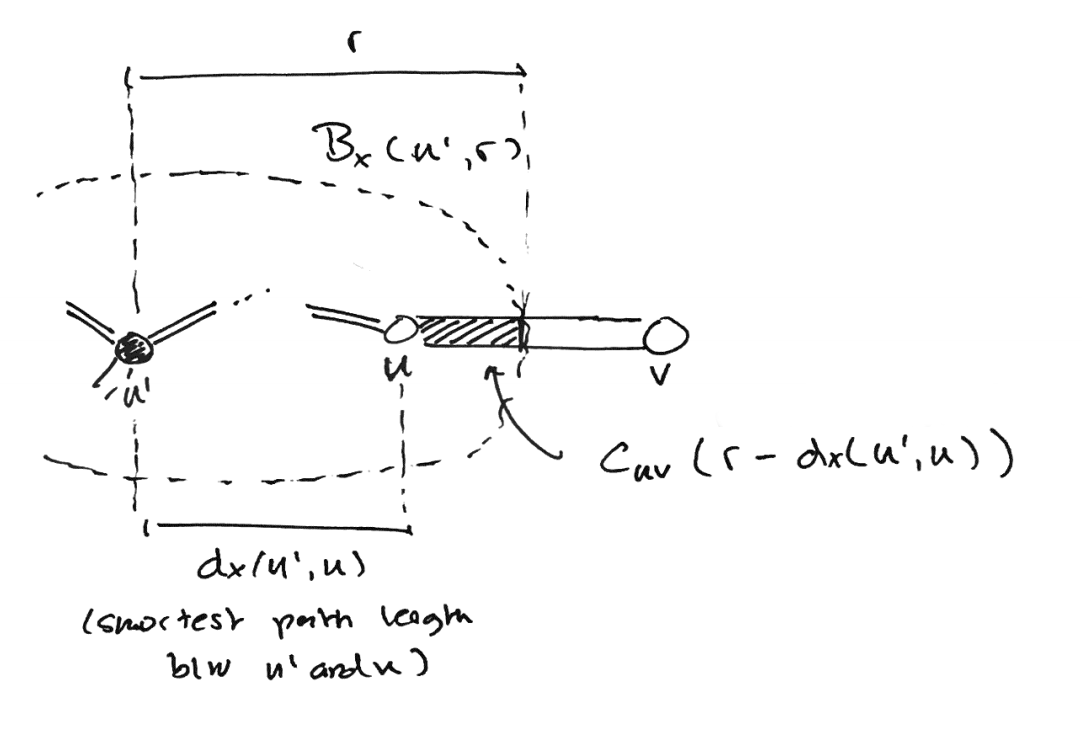
\includegraphics[scale=0.17]{images/image-4.png}
\end{figure}

% --------------------------------------------------------------------
% ROUNDING VIA BALLS
% --------------------------------------------------------------------

\subsection{Rounding via Balls}

Our rounding algorithm will cluster the graph according to appropriately chosen balls. All that remains is to choose the center and radius for each ball. These values will need to be chosen such that each $s_i, t_i$ pair is separated. A certain method of ensuring separation is to center a ball at each $s_i$, then set each radius to $r = 0$. $\mathcal{B}_x(s_i, 0)$ is always the singleton containing $s_i$ thus $s_i$ and $t_i$ are always separated. On the other hand, the ball centered at $s_i$ and with too large a radius may contain both $s_i$ and $t_i$ as we may recall that
\begin{equation*}
d_x(s_i, t_i)
= x_{s_i, t_i}
\geq 1
\end{equation*}

Actually, we can always choose $r < 1$ and ensure that $s_i$ and $t_i$ are not in the same cluster because of the above. However, this does not preclude a ball centered at $s_i$ containing some pair $s_j$ and $t_j$ for $i \neq j$. Consider the following graph whose edges are labeled with the solution to its metric relaxation LP.

\begin{figure}[h!]
\centering
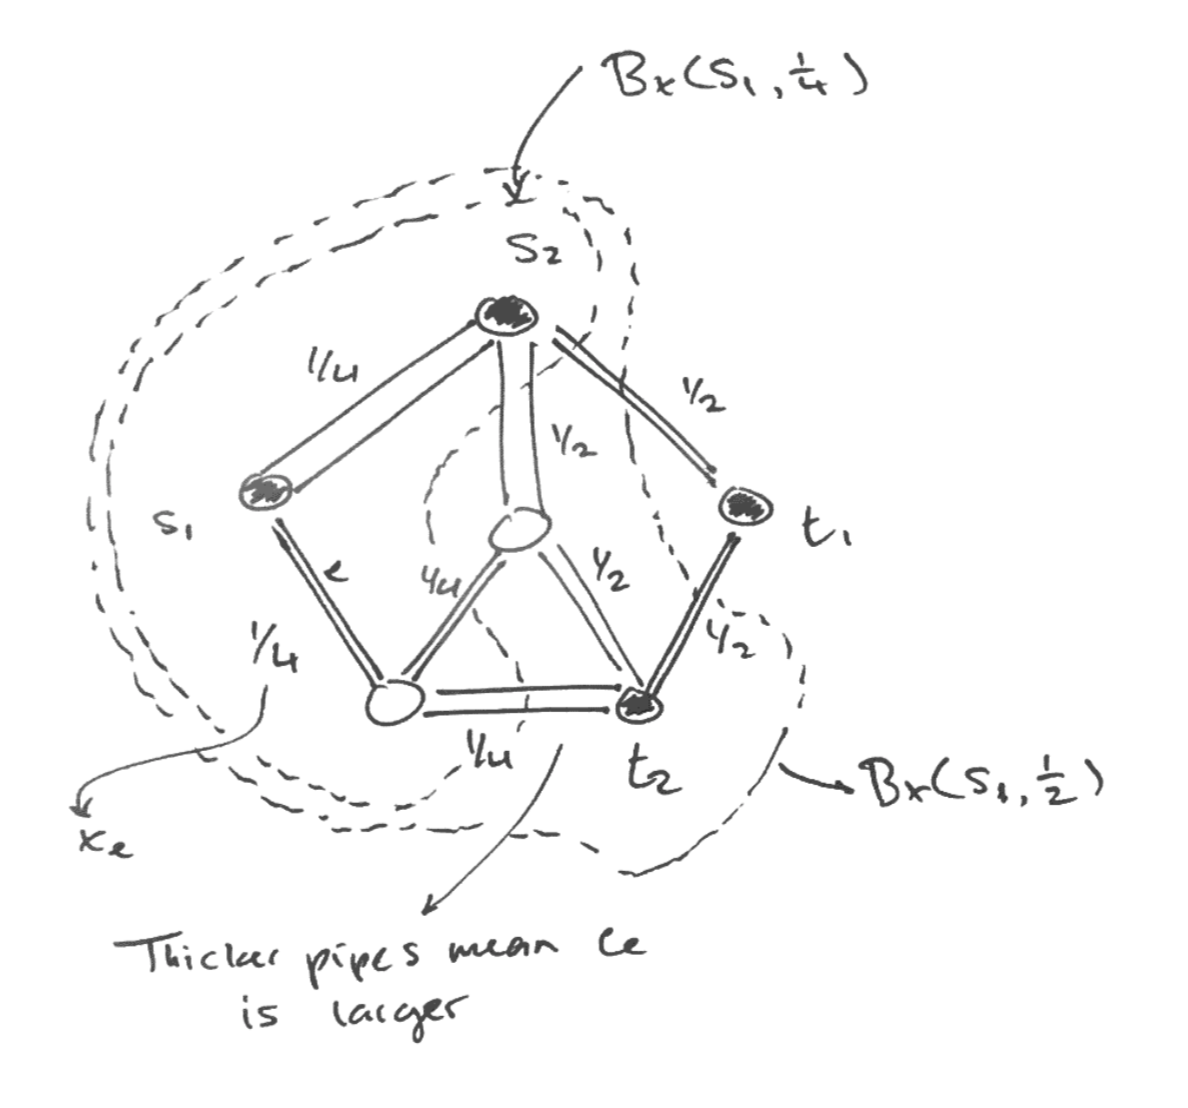
\includegraphics[scale=0.45]{images/image-1.png}
\end{figure}
\vspace{-1em}

Notice that $\mathcal{B}_x(s_1, \frac{1}{2})$ contains both $s_2$ and $t_2$. What is the largest value of $r$ such that a cluster centered at $s_i$ will not contain any $s_j, t_j$ pair? Because $d_x(s_i, t_i) \geq 1$ for any pair $s_i, t_i$, choosing $r < \frac{1}{2}$ suffices because of the triangle inequality. If there is a ball $\mathcal{B}_x(s_i, r)$ where $r < \frac{1}{2}$ containing any $s_j, t_j$, then
\begin{equation*}
x_{s_j, t_j}
= d_x(s_j, t_j)
\leq d_x(s_j, s_i) + d_x(s_i, t_j)
< \frac{1}{2} + \frac{1}{2}
= 1
\end{equation*}

contradicting the fact that $x_{s_j, t_j} \geq 1$. Consequently, any $r < \frac{1}{2}$ will lead the following rounding procedure to return a valid multicut. Notice that in the following procedure, we remove the ball of radius $r$ at each iteration to ensure that no edge is within two different balls.

\noindent\fbox {
\parbox{45.5em} {
\alglabel{alg:rounding}
\textbf{LP Rounding Algorithm}~\thealgorithm

Given $G = (V, E)$, source-sink pairs $\{ (s_i, t_i): i = 1, \ldots, k \}$ and radius $r \in [0, \frac{1}{2})$, do the following:

\begin{quote}
\begin{enumerate}[1.]
\item Solve the linear program relaxation~\ref{eq:metric-lp} for $x$ and set $F = \varnothing$.

\item For $i = 1, \ldots, k$ do:
\begin{enumerate}[-]
\item If $s_i, t_i$ are not separated in $(V, E - F)$, then choose $\mathcal{B}_x(s_i, r)$

\item Update $F = F \cup \partial(\mathcal{B}_x(s_i, r))$

\item Remove vertices in $\mathcal{B}_x(s_i, r)$ and edges in $E(\mathcal{B}_x(s_i, r)) \cup \partial (\mathcal{B}_x(s_i, r))$.
\end{enumerate}

\item Return $F$
\end{enumerate}
\end{quote}
}
}
\vspace{1em}

Now that we have a way of procuring a valid multicut, we can turn our attention towards making it low-cost. Our goal will now be to show that an auspicious choice of $r$ will allow us to bound the cost of the rounded multicut.



% --------------------------------------------------------------------
% BALL GROWING
% --------------------------------------------------------------------
\section{Low-cost Cuts via Ball-Growing}

It will be useful for us to develop some more machinery to discuss the volume of a ball as well as the cost of the partitions added to $F$. Let us define the following.
\vspace{-1em}
\begin{enumerate}[(1)]
\item Define the total volume of the given graph to be $V^*$ given by
\begin{equation*}
V^* = \sum_{e \in E} c_e x_e
\end{equation*}

Since $x$ is the LP optimal solution, $V^*$ lower bounds the cost of the optimal multicut $\opt$.

\item Previously, we defined the volume of a ball $\text{Vol} \; \mathcal{B}_x(u', r)$. Let us now denote another quantity $V_x(s_i, r)$ as the volume of $\mathcal{B}_x(s_i, r)$ with an added $\frac{V^*}{k}$ term.
\begin{equation*}
V_x(s_i, r) = \frac{V^*}{k} + \text{Vol} \; \mathcal{B}_x(s_i, r)
\end{equation*}

The $\frac{V^*}{k}$ term seems a bit mysterious, but adding this term ensures two properties. First, $V_x(s_i, 0) > 0$ for all $i = 1, \ldots, k$ since $\frac{V^*}{k} > 0$. Second, we have
\begin{equation*}
\sum_{i=1}^k V_x(s_i, 0)
= \sum_{i=1} \frac{V^*}{k}
= V^*
\end{equation*}

These two properties will be quite handy later.

\item Define $c_x(s_i, r)$ to be the cost of the cut induced by removing $\mathcal{B}_x(s_i, r)$ from the graph. That is
\begin{equation*}
c_x(s_i, r) = \sum_{e \in \partial(\mathcal{B}_x(s_i, r))} c_e
\end{equation*}
\end{enumerate}

% --------------------------------------------------------------------
% BALL-GROWING
% --------------------------------------------------------------------

\subsection{Ball-Growing}

Consider a the ball $\mathcal{B}(s_i, r)$ removed during an iteration of algorithm~\ref{alg:rounding}. It is uncertain how we can handle the cost of cut $\partial(\mathcal{B}(s_i, r))$ directly, but suppose we could \emph{charge} the cost of the cut to the volume of the ball. That is to say we could discover $\alpha$ such that
\begin{equation}\label{eqn:target-ineq}
c_x(s_i, r) \leq \alpha \cdot V_x(s_i, r)
\end{equation}

This would be very useful as we would then have a potential way to relate the cost of the cut to $V^*$ a lowerbound on $\opt$. The reason why we can expect such an $\alpha$ to exist, and also why pipe networks provide such a nice analogy for this problem, is because the change in volume of a pipe captured by an infinitesimal change in the radius of the ball is proportional to the pipe's cross-sectional area. That is to say:
\begin{equation*}
V_x'(s_i, r) = \frac{d}{dr} V_x(s_i, r) = c_x(s_i, r)
\end{equation*}

Imagine a ball around $s_i$ like so. If we grow $r$ by an infinitesimally small amount then we add the sum of cross-sectional area of all pipes crossing the boundary $\mathcal{B}(s_i, r)$ to the volume of $\mathcal{B}(s_i, r)$. The sum of cross-sectional areas of pipes crossing the boundary of $s_i$'s ball is exactly the quantity measured by $c_x(s_i, r)$!

\begin{figure}[h!]
    \centering
    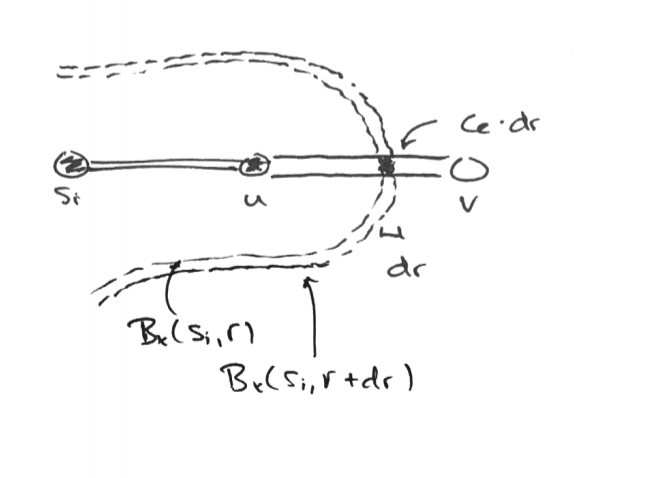
\includegraphics[scale=0.6]{images/image-3.png}
\end{figure}
\vspace{-1em}
Inequality~\ref{eqn:target-ineq} would then reduce to the following
\begin{equation*}
c_x(s_i, r) \leq \alpha \cdot V_x(s_i, r)
\qquad\Longrightarrow\qquad
\frac{c_x(s_i, r)}{V_x(s_i, r)} \leq \alpha
\qquad\Longrightarrow\qquad
\frac{V_x'(s_i, r)}{V_x(s_i, r)} \leq \alpha
\end{equation*}

But $\frac{V_x'(s_i, r)}{V_x(s_i, r)}$ is the derivative of $\ln (V_x'(s_i, r))$. If we let $F'(r) = \frac{V_x'(s_i, r)}{V_x(s_i, r)}$, we can reduced our task of determining $\alpha$ to bounding the value of derivative of $F(r)$. For that we use the Mean Value Theorem. If $F(r)$ is continuous on $[a, b]$ and differentiable on $(a, b)$, then there exists $c \in (a, b)$ such that
\begin{equation*}
F'(c) = \frac{F(b) - F(a)}{b - a}
\end{equation*}

However, $F$ is a monotonic non-increasing function. Thus we have for any $r \in [0, \frac{1}{2})$
\begin{equation*}
F'(r)
\leq \frac{F(\frac{1}{2}) - F(0)}{\frac{1}{2} - 0}
\end{equation*}

Let's first bound $F(\frac{1}{2})$. The volume of any ball of radius $r$ will be at most the total volume of the graph, hence we have the following.
\begin{equation*}
F\bigg( \frac{1}{2} \bigg)
= \ln \bigg( V_x \bigg( s_i, \frac{1}{2} \bigg) \bigg)
\leq \ln\bigg(V^* + \frac{V^*}{k}\bigg)
\end{equation*}

Then we bound $F(0)$. This is where it's critical that $V_x(s_i, 0) > 0$, otherwise the logarithm is undefined!
\begin{equation*}
F(0) = \ln(V_x(s_i, 0)) = \ln\bigg( \frac{V^*}{k} \bigg)
\end{equation*}

We can now bound $F'(r)$. We have
\begin{equation*}
\frac{c_x(s_i, r)}{V_x(s_i, r)}
= F'(r)
\leq \frac{F(\frac{1}{2}) - F(0)}{\frac{1}{2} - 0}
\leq 2 \bigg( \ln\bigg(V^* + \frac{V^*}{k}\bigg) - \ln\bigg( \frac{V^*}{k} \bigg) \bigg)
= 2 \ln(k + 1)
\end{equation*}

What we have shown is that, for an auspicious choice of $r$, we can bound the cost our cut with the volume of the cut. The technique of finding such a cut where we can charge the cost of its boundary to the volume is known as \emph{ball-growing}. To summarize, we have demonstrated
\begin{theorem}\label{thm:region-growing}
Given a feasible solution $x$ to LP~\ref{eq:primal-lp}, for any $s_i$ there exists an $r \in [0, \frac{1}{2})$ that can be found in polynomial time such that
\begin{equation*}
\textup{cost}(\partial(\mathcal{B}_x(s_i, r))) \leq 2 \ln(k+1) \cdot V_x(s_i, r)
\end{equation*}
\end{theorem}

Except we haven't really demonstrated this. The application of the Mean Value Theorem requires $F$ to be differentiable. However, $F(r)$ may not even be continuous at certain points! We will fix this issue with a more careful application of the Mean Value Theorem and also demonstrate how $r$ can be found in polynomial time later on in the notes. For now, let's suppose we have theorem~\ref{thm:region-growing} and complete our analysis of the approximation ratio.

% --------------------------------------------------------------------
% THE APPROXIMATION RATIO
% --------------------------------------------------------------------

\subsection{The Approximation Ratio}

Our heuristic argument in the preceding section demonstrates the existence of an $r$ such that the cost of a ball is at most $2 \ln(k+1)$ times its volume. Using this, we'll show that algorithm~\ref{alg:rounding} returns a $4 \ln(k+1)$-approximation.

\begin{theorem}\label{thm:approx-ratio}
Algorithm~\ref{alg:rounding} returns a $4 \ln(k+1)$-approximation for multicut
\end{theorem}
\begin{proof}
At each iteration of algorithm~\ref{alg:rounding}, we add $F_i = \partial(\mathcal{B}_x(s_i, r))$ to $F$. In iterations $i$ where no ball is removed, we'll let $F_i = \varnothing$ and $\text{Vol} \; \mathcal{B}_x(s_i, r) = 0$. Choosing $r$ according to theorem~\ref{thm:region-growing} gives the cost of $F_i$.
\begin{equation*}
\textup{cost}(F_i)
\leq 2 \ln(k+1) \cdot V_x(s_i, r)
= 2 \ln(k+1) \cdot \bigg( \text{Vol} \; \mathcal{B}_x(s_i, r) + \frac{V^*}{k} \bigg)
\end{equation*}

Since $\mathcal{B}_x(s_i, r)$ is removed from $G$ at every iteration along with all adjacent edges, $F_i \cap F_j = \varnothing$ for $i \neq j$. Additionally, the volume measured by $\text{Vol} \; \mathcal{B}_x(s_i, r)$ will not overlap with that measured by $\text{Vol} \; \mathcal{B}_x(s_j, r)$ for $i \neq j$. The total cost of $F$ returned by the algorithm is the following.
\begin{align*}
\textup{cost}(F)
&= \sum_{i=1}^k \textup{cost}(F_i) \\
&\leq 2 \ln(k+1) \cdot \sum_{i=1}^k \bigg( \text{Vol} \; \mathcal{B}_x(s_i, r) + \frac{V^*}{k} \bigg) \\
&= 2 \ln(k+1) \cdot \big( V^* + V^* \big) \\
&= 4 \ln(k+1) \cdot V^*
\end{align*}

and because $V^*$ is the cost of the optimal LP solution $x$, which lower bounds the optimal cost $\opt$ of any multicut, we have $\textup{cost}(F) \leq 4 \ln(k+1) \cdot \opt$ as required.
\end{proof}

% --------------------------------------------------------------------
% CONTINUITY ISSUES
% --------------------------------------------------------------------

\subsection{Fixing Continuity Issues}

Let's revisit the continuity of $F(r) = \ln(V_x(s_i, r))$ and ask where $F(r)$ could be discontinuous. Around where $r = d_x(s_i, u)$ for some vertex $u \neq s_i$, there could be a discontinuous jump in $V_x(s_i, r)$ because $u$ could be connected to more than one pipe not currently in $\mathcal{B}_x(s_i, r)$.
\begin{figure}[h!]
    \centering
    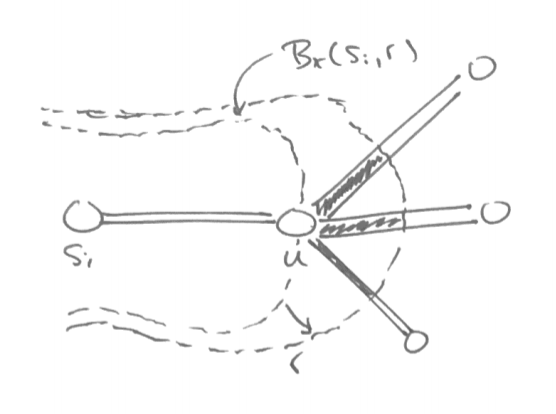
\includegraphics[scale=0.6]{images/image-2.png}
\end{figure}
\vspace{-1em}

However, on intervals of $r \in [0, \frac{1}{2})$ where increasing $r$ does not introduce a new vertex into $\mathcal{B}_x(s_i, r)$, the value of $V_x(s_i, r)$ grows smoothly with respect to $r$. This suggests that we should partition the interval $[0, \frac{1}{2})$ into intervals where \emph{no new vertex} is introduced into $\mathcal{B}_x(s_i, r)$. We now prove theorem~\ref{thm:region-growing}.

\begin{proof}[Proof of theorem~\ref{thm:region-growing}]
We will show that there exists $r \in [0, \frac{1}{2})$ such that
\begin{equation*}
\frac{c_x(s_i, r)}{V_x(s_i, r)} \leq 2 \ln(k+1)
\end{equation*}

Let us order the vertices $v \neq s_i$ as $v_1, \ldots, v_{\ell}$ where
\begin{equation*}
d_x(s_i, v_{j_1}) \leq d_x(s_i, v_{j_2})
\end{equation*}

when $j_1 \leq j_2$, define $r_j = d_x(s_i, v_j)$, and denote $r_j^-$ as value that's infinitesimally smaller than $r_j$. We will demonstrate the existence of $r$ by choosing it uniformly at random on the interval $[0, \frac{1}{2})$. If we can bound the \emph{expectation} of $\frac{c_x(s_i, r)}{V_x(s_i, r)}$ by what we want, then there must exist an actual choice of $r$ where the bound holds deterministically. Our choice of partitioning $[0, \frac{1}{2})$ using $r_j$'s is critical as $F(r)$ is continuous over interval $[r_j, r_{j+1}^{-}]$ and differentiable over $(r_j, r_{j+1}^-)$. For notational simplicity, let $r_{\ell + 1} = \frac{1}{2}$. Let us compute the expectation of $\frac{c_x(s_i, r)}{V_x(s_i, r)}$ when $r$ is distributed uniformly at random on $[0, \frac{1}{2})$.
\begin{align*}
\mathbb{E} \bigg[ \frac{c_x(s_i, r)}{V_x(s_i, r)} \bigg]
&= \frac{1}{\frac{1}{2} - 0} \cdot \int_0^{\frac{1}{2}} \frac{c_x(s_i, r)}{V_x(s_i, r)} \; dr \\
&= \frac{1}{\frac{1}{2} - 0} \cdot \sum_{j = 1}^{\ell} \int_{r_j}^{r_{j+1}^-} \frac{c_x(s_i, r)}{V_x(s_i, r)} \; dr \\
&= 2 \cdot \sum_{j=1}^\ell \Big( \ln(V_x(s_i, r^-_{j+1})) - \ln(V_x(s_i, r_{j})) \Big) \\
&\leq 2 \cdot \sum_{j=1}^\ell \Big( \ln(V_x(s_i, r_{j+1})) - \ln(V_x(s_i, r_{j})) \Big)
\end{align*}

The last line follows as $F(r)$ is monotonically non-decreasing. This forms a telescoping sum which reduces to
\begin{equation*}
2 \cdot \sum_{j=1}^\ell \Big( \ln(V_x(s_i, r_{j+1})) - \ln(V_x(s_i, r_{j})) \Big)
= 2 \cdot \Big( \ln(V_x(s_i, \tfrac{1}{2})) - \ln(V_x(s_i, 0)) \Big)
\leq 2 \ln(k+1)
\end{equation*}

Consequently, the expectation is bounded by $2 \ln(k+1)$ hence there must be an $r$ achieving $\frac{c_x(s_i, r)}{V_x(s_i, r)} \leq 2 \ln(k+1)$. To find $r$ in polynomial time, observe that on the interval $[r_j, r_{j+1}]$ the cost of the boundary $c_x(s_i, r)$ remains constant while $V_x(s_i, r_{j+1})$ grows monotonically. This means the ratio $\frac{c_x(s_i, r)}{V_x(s_i, r)}$ is minimized at $r_{j+1}$. Finding the minimizer requires only checking each $r_1, \ldots, r_{\ell}$, and as $\ell \leq n$, a linear number of computations suffice.
\end{proof}



% --------------------------------------------------------------------
% CONCLUSION
% --------------------------------------------------------------------
\section{Conclusion}

In this note, we introduced the graph Laplacian as a matrix that was reverse engineered to encode cut sizes in its quadratic form. We did so for two reasons: (1) maximizing the quadratic form would provide a relaxation of the maxcut problem, and (2) doing so would hopefully allow the spectrum of the Laplacian, via the variational characterization of eigenvalues, to capture some combinatorial structure of the graph. Indeed, we verified that the spectrum of the Laplacian held a nice connection to various extremal graph properties.
\vspace{-1em}
\begin{enumerate}[-]
  \item We saw that $\lambda_2 = 0$ if the graph is disconnected.

  \item We saw that $\lambda_k = 0$ if the graph has $k$ disjoint connected components.

  \item We saw that $\lambda_n = 2d$ if a $d$-regular graph is bipartite.
\end{enumerate}

However, we have not fully discussed where relaxations come into play. Revisiting how we wrote the Rayleigh quotient for $\lambda_n$
\begin{equation*}
\frac{x^\top L_G x}{x^\top x}
= 2d - \frac{\sum_{(i, j) \in E} \big( x(i) + x(j) \big)^2 }{\sum_{i \in V} x(i)^2}
\end{equation*}

If $\lambda_n$ is large then $x(j)$ should be close to $-x(i)$ for each $(i, j) \in E$. This means that $G$ should have a large maxcut, or rather, be ``close'' to being bipartite. What this suggests is our next big idea: the eigenvalues of the Laplacian provide a robust way of continuously measuring certain combinatorial properties of a graph!


\bibliographystyle{plain}
\begin{thebibliography}{99}
\bibitem{ARV09}
Arora, S., Rao, S., \& Vazirani, U. (2009). ``Expander flows, geometric embeddings and graph partitioning.'' In \emph{Journal of the ACM (JACM)}, 56(2), 5.

\bibitem{CKKRS06}
Chawla, S., Krauthgamer, R., Kumar, R., Rabani, Y., \& Sivakumar, D. (2006). ``On the hardness of approximating multicut and sparsest-cut.'' In \emph{computational complexity}, 15(2), 94-114.

\bibitem{GVY96}
Garg, N., Vazirani, V. V., \& Yannakakis, M. (1996). ``Approximate max-flow min-(multi) cut theorems and their applications.'' In \emph{SIAM Journal on Computing}, 25(2), 235-251.

\bibitem{KM09}
Kelner, J. A., \& Madry, A. (2009, October). ``Faster generation of random spanning trees''. In \emph{2009 50th Annual IEEE Symposium on Foundations of Computer Science} (pp. 13-21). IEEE.

\bibitem{LR88}
Leighton, T., \& Rao, S. (1988). ``An approximate max-flow min-cut theorem for uniform multicommodity flow problems with applications to approximation algorithms.'' In \emph{[Proceedings 1988] 29th Annual Symposium on Foundations of Computer Science}. (pp. 422-431). IEEE.

\bibitem{LR99}
Leighton, T., \& Rao, S. (1999). ``Multicommodity max-flow min-cut theorems and their use in designing approximation algorithms.'' In \emph{Journal of the ACM (JACM)}, 46(6), 787-832.

\bibitem{Tre05}
Trevisan, L. (2005). ``Approximation algorithms for unique games.'' In \emph{46th Annual IEEE Symposium on Foundations of Computer Science} (pp. 197-205). IEEE.
\end{thebibliography}

\end{document}
